\documentclass[a4paper, 12pt]{article}
\usepackage[top=1cm, bottom = 2cm, left = 2cm, right = 2cm]{geometry}
\usepackage[utf8]{inputenc}
\usepackage[brazil]{babel}
\usepackage{listings}
\usepackage[framed, numbered]{matlab-prettifier}
\usepackage[T1]{fontenc}
\usepackage{indentfirst}
\usepackage{graphicx}
\usepackage{epstopdf}
\usepackage{float}
\usepackage{amsmath}
\usepackage{amssymb}
\usepackage{systeme}

\title{Exercício 1 - Aula 8 \\ EET-01}

\author{
  Igor Caldeira Magalhães\\igorcmag@gmail.com
}
\date{16 de maio de 2020}

\begin{document}
\maketitle
\section{Enunciado}

Considere os sinais x(t) dados pelos sinais wave (em anexo).

- Obtenha os sinais x[n] utilizando o conversor AD disponibilizado.

- Aplique a transformada de Fourier de Tempo Discreto em x[n].

Qual é a frequência máxima do sinal x[n]?

Qual deve ser a frequência de amostragem mínima para assegurar que o sinal possa ser recuperado posteriormente por um processo de filtragem em banda base?

%O exercício deve ser entregue: Documento simples deve ser apresentado, contendo o seguinte conteúdo:
%Nome da disciplina;
%Nome do aluno;
%Enunciado do exercício;
%Figuras obtidas - Com breve descrição: A Figura xx mostra ...
%Código .m e breve descrição do código matlab (octave);

\section{Solução}

Primeiramente, extraiu-se o arquivo de audio \textit{Blackbird.wav} para um vetor $x[n]$, bem como a frequência com que o arquivo de áudio foi gravado $f_s = 1/T = 44.100 Hz$. O gráfico de $x[n]$ é apresentado na \textbf{figura 1}. Em seguida, calculou-se a transformada de Fourier em tempo discreto de $x[n]$, plotou-se seu gráfico, \textbf{figura 2}, e obteve-se o valor de $\omega_B $ para a largura de banda. A \textbf{frequência de Nyquist} $f_0$ é dada por 

$$f_0 = \frac{\omega_B f_s}{2\pi} \thickapprox \frac{0,2\cdot 44100}{2\pi} \thickapprox 1.400 Hz$$

Assim, para que o sinal analógico possa ser convertido para o modo digital (e gravado no computador) de forma reversível, é necessário que a taxa de amostragem seja no mínimo de $2.800 Hz$. Como o arquivo de áudio foi gravado com uma frequência de $44.100 Hz$, é possível o reverter a gravação para o modo analógico (ou seja, emitir novamente o "som físico") sem perdas.

\lstinputlisting[style=Matlab-editor, caption={Codigo em MATLAB que realiza as tarefas descritas.}, basicstyle = \mlttfamily\scriptsize]{ex1.m}

\begin{figure}[H]
	\centering
	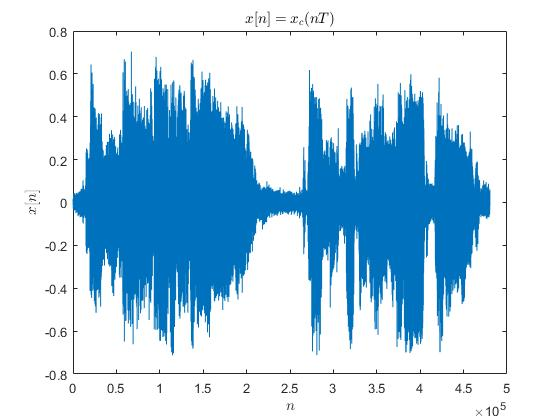
\includegraphics[scale=0.7]{img1.jpg} 
	\caption{Gráfico de $x[n]=x_c(nT)$ para o arquivo \textit{Blackbird.wav}.}
	\label{fig:1}
\end{figure}

\begin{figure}[H]
	\centering
	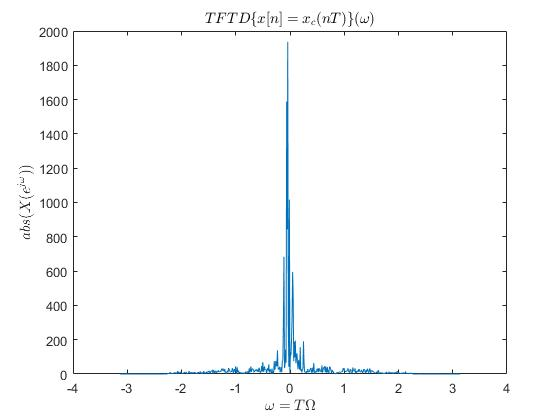
\includegraphics[scale=0.7]{img2.jpg} 
	\caption{Gráfico da transformada de Fourier em tempo discreto de  $x[n]=x_c(nT)$ para o arquivo \textit{Blackbird.wav}.}
	\label{fig:2}
\end{figure}

A análise do arquivo \textit{smariosong.wav} é idêntica. As frequências de amostragem e Nyquist obtidas foram, respectivamente, $f_s= 44.100 Hz$ e $f_0= 4.200 Hz$. O resultados estão expressos na \textbf{figura 3} e \textbf{figura 4}.

\begin{figure}[H]
	\centering
	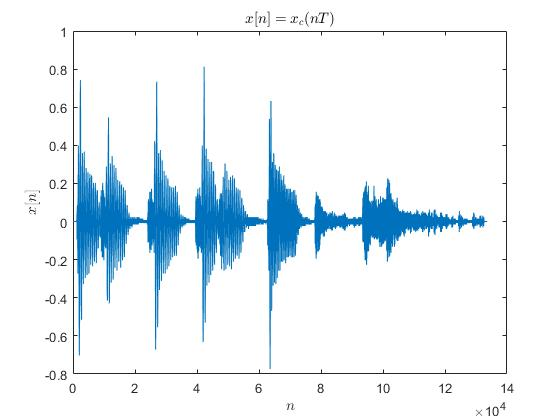
\includegraphics[scale=0.7]{img3.jpg} 
	\caption{Gráfico de $x[n]=x_c(nT)$ para o arquivo \textit{smariosong.wav}.}
	\label{fig:3}
\end{figure}

\begin{figure}[H]
	\centering
	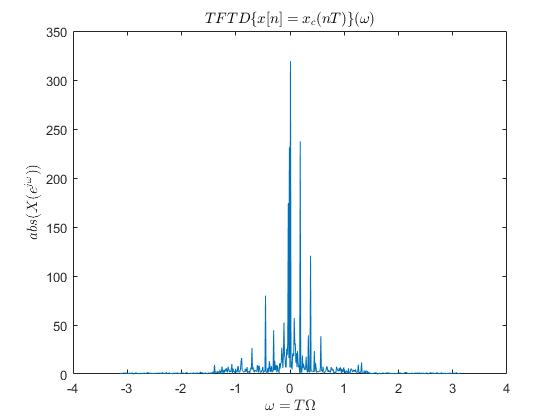
\includegraphics[scale=0.7]{img4.jpg} 
	\caption{Gráfico da transformada de Fourier em tempo discreto de  $x[n]=x_c(nT)$ para o arquivo \textit{smariosong.wav}.}
	\label{fig:4}
\end{figure}
\end{document}